\documentclass[a4paper,11pt]{article}
\usepackage[utf8]{inputenc}
\usepackage[paper=a4paper, hmargin=1.5cm, bottom=1.5cm, top=3.5cm]{geometry}
\usepackage[T1]{fontenc}
\usepackage[colorlinks=true, linkcolor=blue]{hyperref} %Links para el indice.
\usepackage{amsfonts}
\usepackage{verbatim}
\usepackage{listings}
\usepackage{caption}
\usepackage{subcaption}
\usepackage{graphicx}
\usepackage{wrapfig}
\usepackage[section]{placeins}
\usepackage{float}
%\usepackage{adjustbox}
\usepackage{amsmath}
\usepackage{blindtext}
\usepackage{sidecap}
\usepackage{color}

\captionsetup[subfigure]{labelformat=empty}

% \newcommand{\real}{\hbox{\bf R}}

\newcommand{\rto}{\textit{rto}}
\newcommand{\rtt}{\textit{rtt}}

\title{Conexiones}

\begin{document}

\maketitle

\begin{center}
	Universidad de Buenos Aires - Departamento de Computaci\'on - FCEN
\end{center}

\vspace{2cm}
Integrantes:

\begin{itemize}
	\item Gallardo, Guillermo L.U.: 32/10 \verb+gagdiez.c@gmail.com+
	\item Fixman, Martin L.U.: 391/11 \verb+martinfixman@gmail.com+
	\item Matayoshi, Leandro L.U.: 79/11 \verb+leandro.matayoshi@gmail.com+
	\item Szyrej, Alexander L.U.: 642/11 \verb+alexander.szyrej@gmail.com+

\end{itemize}

\newpage

\tableofcontents

\newpage

\section{Introducci\'on}
    
    Los protocolos confiables de transporte permiten al usuario abstraerse 
    de los problemas de transmisi\'on de la red, por ej, el protocolo TCP 
    nos permite enviar mensajes a traves de medios que pierden, desordenan
    y modifican paquetes. 
    
    El protocolo PTC es una implementaci\'on de la catedra, el mismo est\'a 
    basado en TCP, por lo tanto, intenta asegurar que los paquetes lleguen de un
    punto a otro utilizando diversos mecanismos como control de flujo, realizar
    la conexi\'on en etapas, mantener una ventana deslizante para enviar 
    y recibir paquetes, etc. 
        
    En este trabajo estudiaremos como se comporta PTC, poniendo especial 
    atenci\'on a la retransmisi\'on de paqutes. Para ello 
    primero emularemos escenarios donde existan delay y perdida
    de paquetes entre dos nodos comunicados. Luego, iremos modificando
    par\'ametros de la implementaci\'on para ver como ello afecta el reenvio 
    de paquetes. 


\section{M\'etodos}

    El protocolo PTC utiliza un sistema de \textit{acknowledge} para
    saber si un paquete fue recibido. En caso de no recibir un \textit{ack}
    para un  determinado paquete luego de un umbral de tiempo, procede a
    retransmitirlo. Dicho umbral, denominado \textit{rto} se va estimando
    a medida que se reconocen los paquetes enviados usando las
    siguientes funciones:

        $$RTTVAR = (1-\beta)RTTBAR + \beta |SRTT-RTT|$$
        $$SRTT = (1-\alpha)SRTT + \alpha RTT$$
        $$RTO = SRTT + max( 1, K * RTTVAR) $$

    Donde $K, \alpha, \beta \in \mathbb{Q}$, $RTT$ es el valor de
    \textit{rtt} calculado para el \'ultimo \textit{ack} recibido.
    En la implementaci\'on utilizada se inicializan los valores de la
    siguiente manera: $K = 4, \alpha={{1}\over{8}}$,
    $\beta={{1}\over{4}}$, $SRTT={RTT_0}$, $RTTVAR={{RTT}\over{2}}$.
    Siendo $RTT_0$ el primer \textit{rtt} calculado.

\subsection{Sistema}

	Tanto el cliente como el servidor est\'an simulados en el mismo sistema. La
	topolog\'ia de este sistema es similar a la de dos equipos, un cliente y un
	servidor, conectados mediante un link ethernet en la misma red o en
	diferentes redes pero con cierto nivel previsible de congesti\'on.

	Al protocolo PTC se le puede artificialmente poner un \emph{delay} ficticio,
	que simular\'ia tanto la distancia que hay entre en cliente y el servidor en
	la red simulada como el nivel de congesti\'on entre estos dos puntos.
  Por ejemplo, en los entornos reales (muy distintos al de nuestra experimentaci\'on),
  el delay incluye el tiempo en el que
  los paquetes permanecen en los buffers de cada router antes de ser forwardeados,
  el cual puede ser un factor a tener en cuenta para medir el nivel de congesti\'on
  de una red.
	Tambi\'en se tiran adrede los paquetes con una probabilidad $p$, simulando
	la perdida de paquetes que puede pasar en una red congestionada o con links
	erroneos.

	Dada la velocidad de procesamiento actual, sumado al procesamiento en
	paralelo, podemos asumir que el RTT real es el delay ficticio que generamos,
	dado que un tick simulado ronda el orden del mill\'on de tick reales.

	En lo que respecta a este TP, todas las conexiones son conexiones que usan
	el protocolo PTC.

\newpage
\section{Desarrollo}

    En primera instancia se implementaron dos scripts en python que 
    actuan uno como cliente y otro como servidor.
    Luego, se modific\'o la implementaci\'on de PTC para poder simular
    delay y perdida de paquetes (el contexto de una red), adem\'as de transformar en par\'ametros
    a los valores $\alpha$ y $\beta$ para estudiar como se modifica el
    \rto{} en base a los mismos.  

  \subsection{Modificaciones a la Implementaci\'on}
    Se agregaron al sistema variables para manejar la probabilidad de que 
    un paquete se pierda en el env\'io, el delay antes de contestar con 
    un ACK, el valor de $\alpha$ y $\beta$.

    \subsubsection{rto}
    Se modific\'o para que los valores de $\alpha$ y $\beta$ fueran 
    variables seteables al momento de inicializar el \textit{RTOEstimator}.
    
    \subsubsection{protocol}
    Se modific\'o la incializaci\'on, ahora recibe los par\'ametros 
    $\alpha$, $\beta$, \textit{perdida} y \textit{delay}.
    
    $\alpha$, $\beta$ se utilizan para inicializar el \textit{RTOEstimator}.
    
    Se modific\'o el m\'etodo \textit{send\_and\_queue}, ahora, espera 
    \textit{delay} ticks antes de enviar el paquete con una probabilidad
    de $1-perdida$. En una primera instancia se intent\'o incluir el delay
    en la funci\'on \textit{send\_ack} del m\'odulo \textit{handler}, pero
    en la experimentaci\'on notamos que ciertos valores de \textit{rtt estimado}
    quedaban muy por debajo del delay seteado, por lo tanto entendimos que 
    algunos acks nos evad\'ian, y se mandaban por otro m\'etodo. 
    Dado que el paquete se trackea antes del delay en \textit{send\_and\_queue},
    el cliente interpreta el tard\'io ack como una demora en la red y calcula el 
    rtt/rto en base a esa demora.

    Se modific\'o tambi\'en el m\'etodo \textit{free} para que imprima el \rto{} 
    estimado durante la conexi\'on.        
    
    \subsubsection{ptc\_socket}
    Se modific\'o el wrapper, ahora se debe inicializar con valores para 
    $\alpha$, $\beta$, \textit{perdida} y \textit{delay}, los mismos son
    utilizados al momento de crear el objeto \textit{PTCProtocol} del 
    paquete \textit{protocol}.
    
    Se cre\'o el m\'etodo \textit{alumnos\_change\_delay} que recibe un
    entero y cambia el delay de la conexi\'on mediante el m\'etodo nuevo
    puesto en \textit{protocol}.
    
  \subsection{Experimentaci\'on}  
    Para estudiar el comportamiento de PTC realizaremos los siguientes
    experimentos:
    
    \emph{Convergencia de RTO:} Queremos ver si el valor de \rto{} se
    estabiliza luego de enviar un gran n\'umero de paquetes.
  
    \emph{Valor de RTO variando $\beta$:}
    
    \emph{Valor de RTO variando $\alpha$:}
    
    \emph{Valor de RTO cuando la red se congestiona de golpe:} En este
    caso queremos ver que sucede cuando la red esta operando normalmente
    y de repente subimos mucho el delay.

\newpage
\section{An\'alisis y Resultados}

    \subsection{Valor de RTO variando $\alpha$ y $\beta$}
    
        Primero estudiamos como var\'ia el \rto{} cuando se utilizan los
        valores extremos de $\alpha$ y $\beta$. Se utiliz\'o un valor 
        de delay = \textit{6 ticks} sin probabilidad de p\'erdida.

        Puede verse en la \textit{Figura 1}, que tomando $\alpha=0$, 
        $\beta=0$ los cálculos ignoran por completo los nuevos 
        valores de RTT y consideran únicamente los valores de SRTT
        anteriores. En este caso, el valor constante inicial.

        La \textit{Figura 2} muestra como al tomar ambas variables el valor
        1, los cálculos ignoran los valores anteriores (tanto de variación
        de RTT (RTTVAR) como de SRTT), y modifican los resultados
        únicamente en función de la última muestra de RTT obtenida. El
        resultado es un gráfico en donde el RTO coincide exactamente con
        el SRTT, y ambos responden excesivamente a cualquier fluctuación
        que se produzca en el valor del RTT.
    
        Por otra parte, la \textit{Figura 3} muestra lo que sucede al 
        ponderar de igual manera los valores anteriores con los nuevos, al
        tomar ambas variables con valor 0.5. Esto debería generar valores
        cercanos a los de las muestras anteriores, pero que sean capaces
        de responder a cambios significativos y permanentes del valor de
        RTT. En otras palabras, que alcancen un equilibrio entre ambas
        propuestas. Sin embargo, el comportamiento no fue el esperado. 
        
        El resultado es una serie de cálculos demasiado sensibles a las
        fluctuaciones temporales que responden excesivamente a estos
        cambios. Por ello hicimos una \'ultima prueba (\textit{Figura 4})
        donde fijamos el valor de $\alpha$ en 0.15 y $\beta$ en 0.20 
        (cercanos al propuesto por el RFC 6298).
        Las conexiones en las distintas redes por lo general permanecen
        estables la mayor parte del tiempo, por lo que los cambios bruscos
        de \rtt{} son poco probables. Por otro lado el valor de $\beta$ 
        permite agregar un poco de sensibilidad a los cambios en el valor
        de los \textit{rtts}.

        \begin{figure}[H]
	    \center
	    \begin{subfigure}{0.48\textwidth}
		    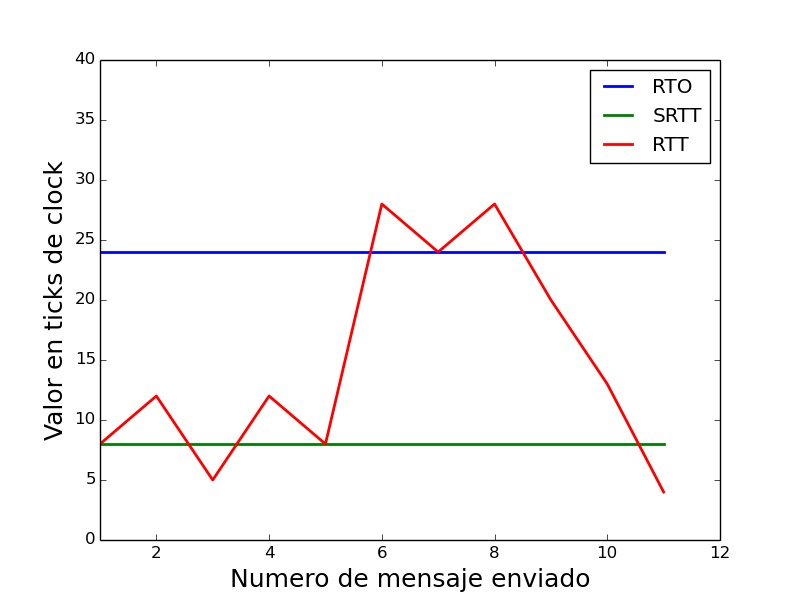
\includegraphics[width=1.0\textwidth]{imagenes/test_0_0.jpg}
		    \caption{Figura 1}
	    \end{subfigure}
	    ~
	    \begin{subfigure}{0.48\textwidth}
		    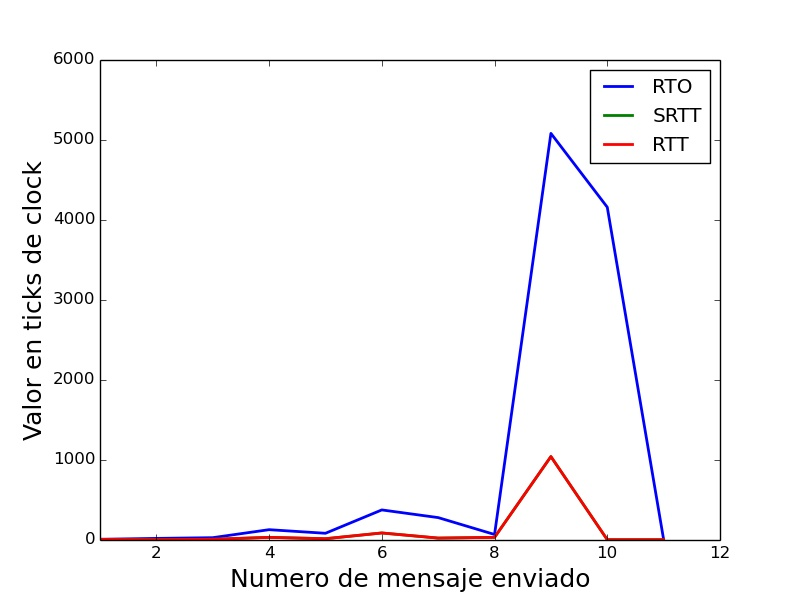
\includegraphics[width=1.0\textwidth]{imagenes/test_1_1.jpg}
		    \caption{Figura 2}
	    \end{subfigure}
	    \end{figure}    

        \begin{figure}[H]
	    \center
	    \begin{subfigure}{0.48\textwidth}
		    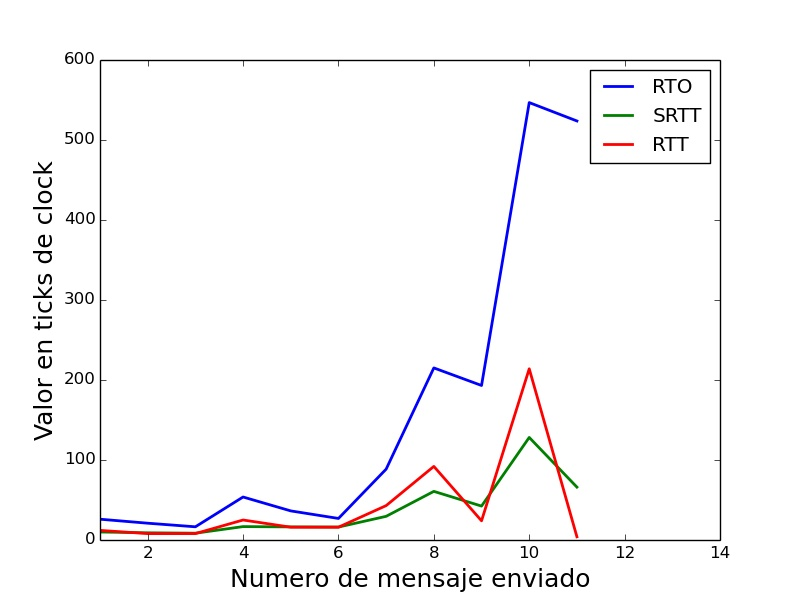
\includegraphics[width=1.0\textwidth]{imagenes/test_5_5.jpg}
		    \caption{Figura 3}
	    \end{subfigure}
	    ~
	    \begin{subfigure}{0.48\textwidth}
		    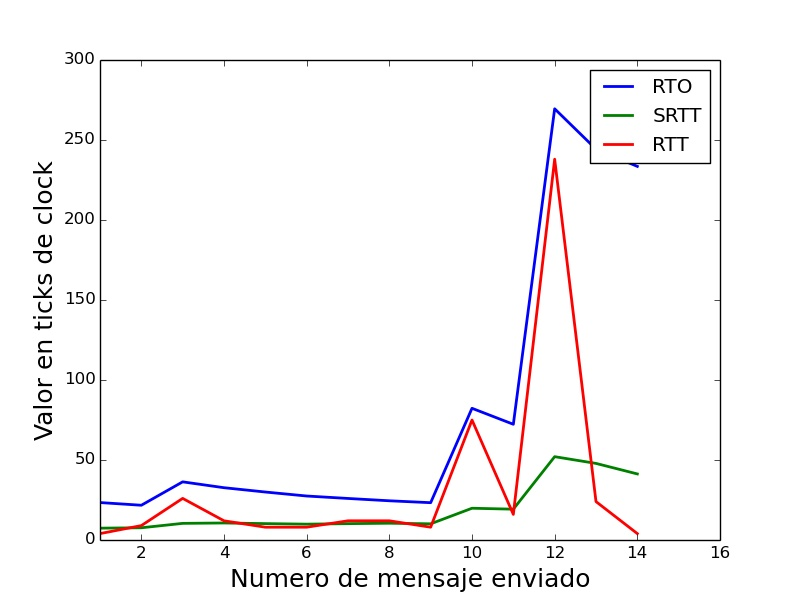
\includegraphics[width=1.0\textwidth]{imagenes/test_a_b.jpg}
		    \caption{Figura 4}
	    \end{subfigure}
	    \end{figure}    
	       
        Finalmente intentamos medir muchos valores de \rto{} para 
        diversas convinaciones de $\alpha$ y $\beta$. 
        Los resultados de medir el \rto{} para un valor fijo de 
        \textit{25 ticks} y probabilidad de perdida cero luego de 
        enviar 200 paquetes se pueden ver en la \emph{Figura 4}.
        
    \subsection{Perdida de paquetes variando $\alpha$ y $\beta$}
        Para estudiar la perdida de paquetes se fij\'o el valor de 
        de \rto{} en \textit{25 ticks} y no se simularon p\'erdidas.
        Sin embargo en varios casos hubo retransmisiones, la 
        \textit{Figura 5} muestra el resultado para el env\'io de 150
        paquetes mientras que la \textit{Figura 6} lo muestra para 300.
        
    \begin{figure}[H]
	    \center
	    \begin{subfigure}{0.32\textwidth}
		    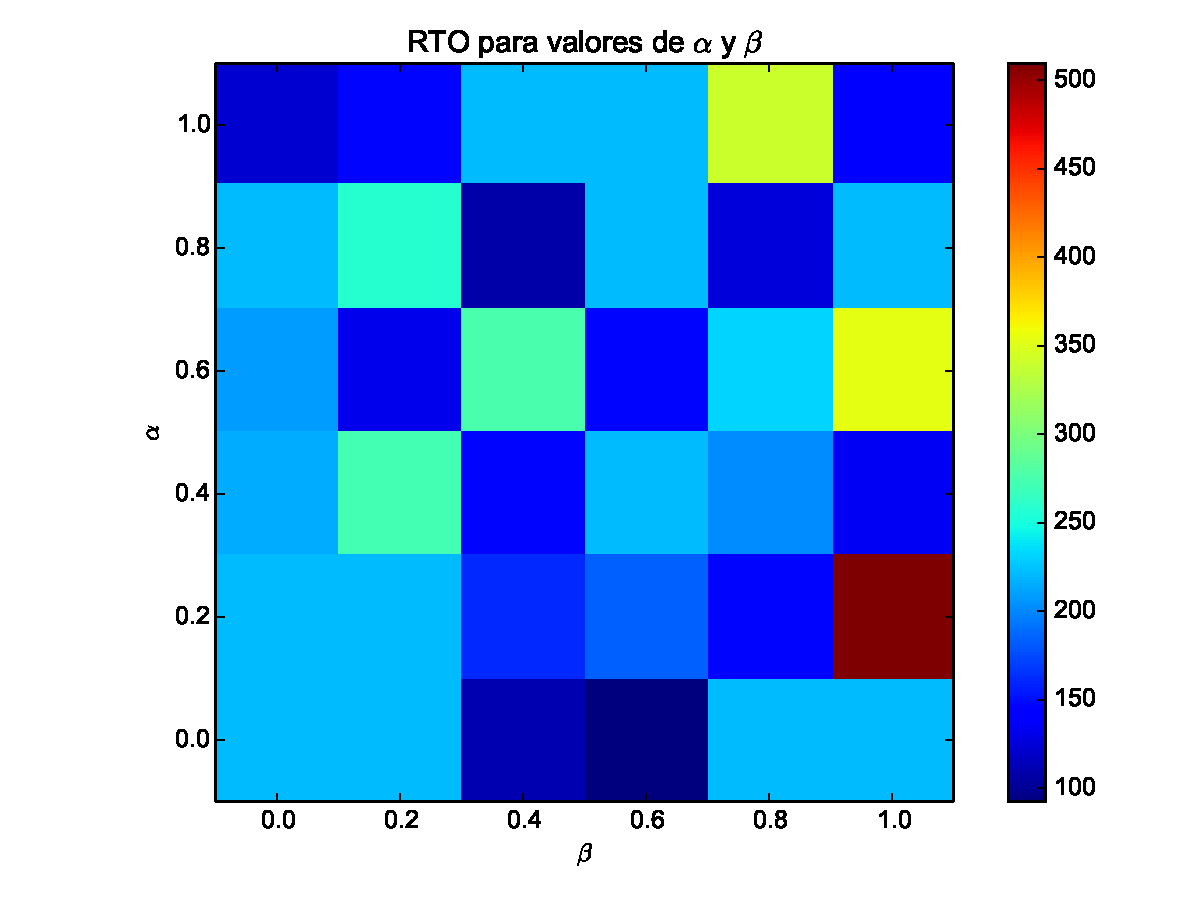
\includegraphics[width=1.0\textwidth]{imagenes/rto_vs_alphaBeta.pdf}
		    \caption{Figura 4}
	    \end{subfigure}
	    ~
	    \begin{subfigure}{0.32\textwidth}
		    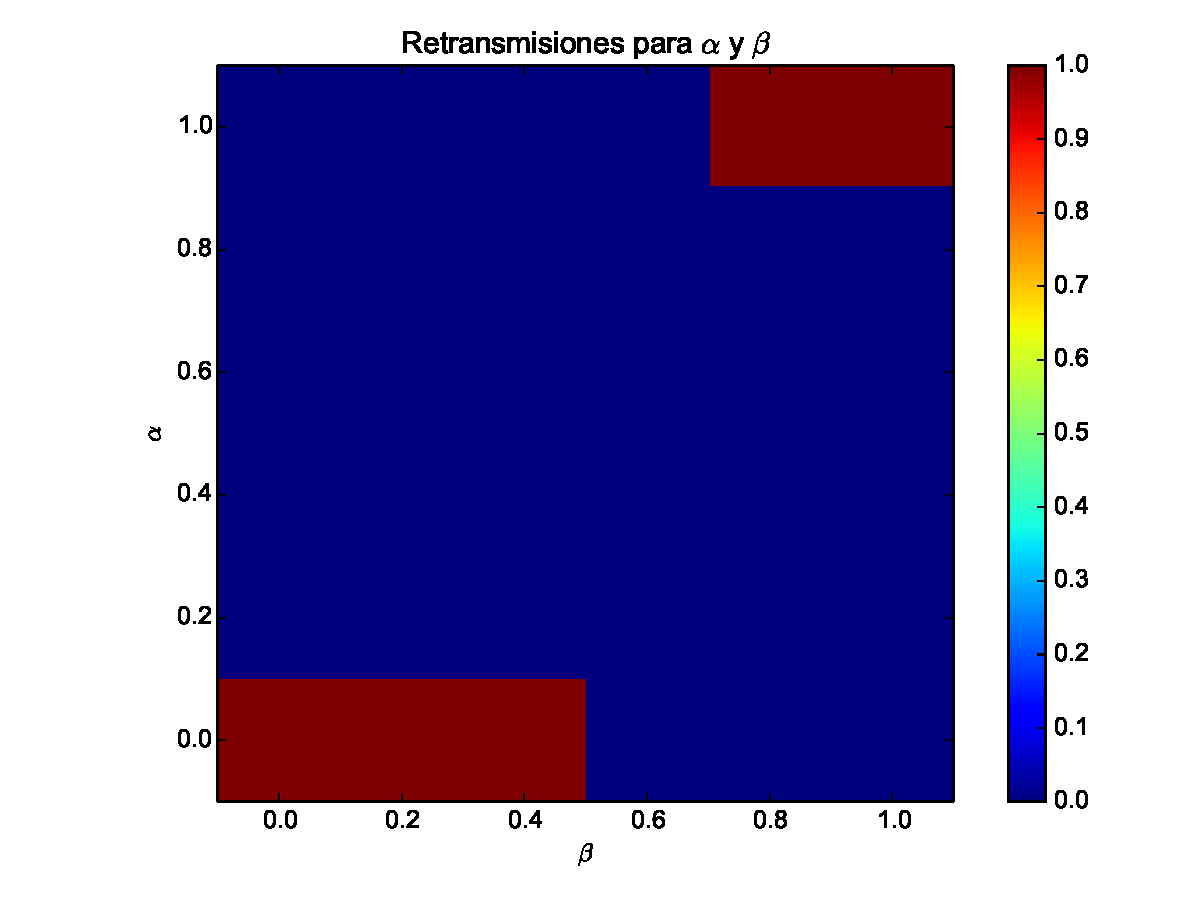
\includegraphics[width=1.0\textwidth]{imagenes/retransmisiones_150.pdf}
		    \caption{Figura 5}
	    \end{subfigure}
	    ~
	    \begin{subfigure}{0.32\textwidth}
		    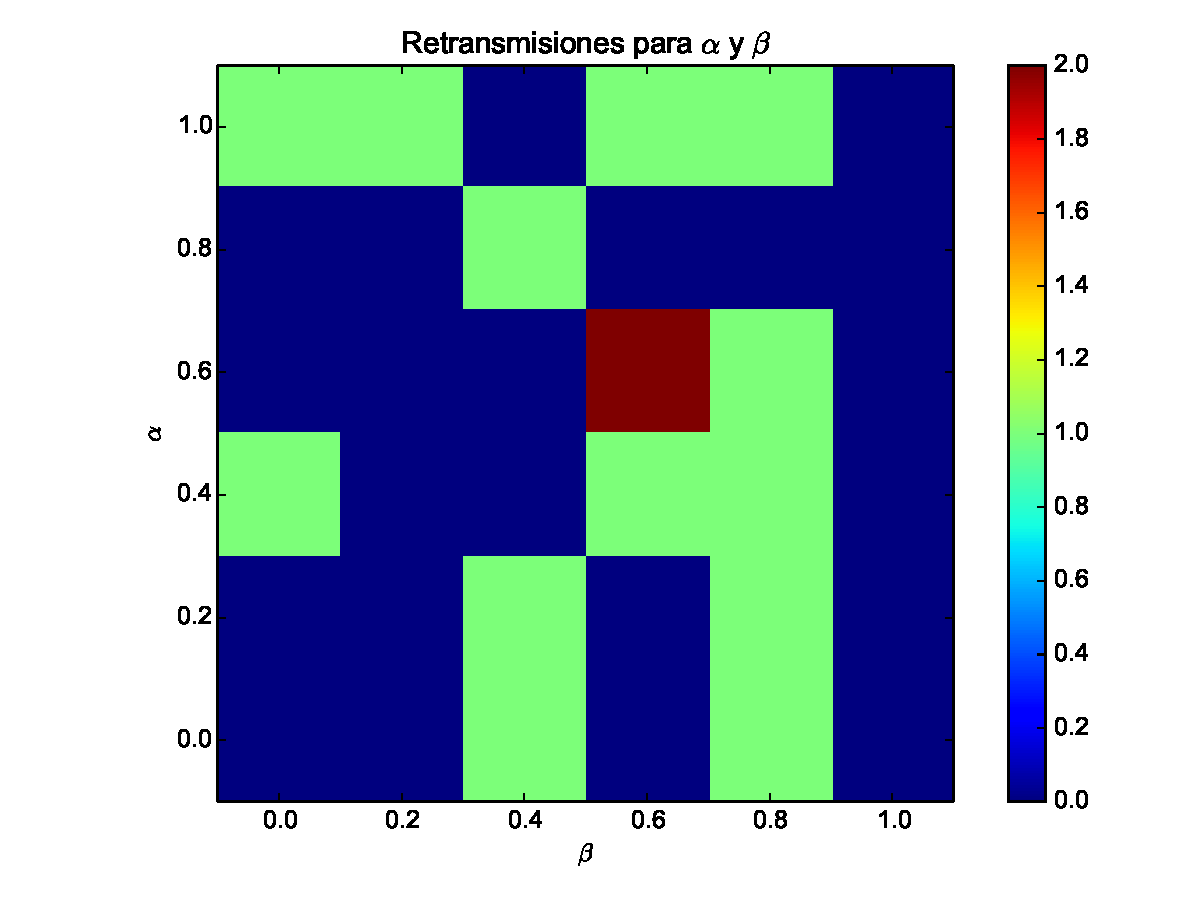
\includegraphics[width=1.0\textwidth]{imagenes/retransmisiones_300.pdf}
		    \caption{Figura 6}
	    \end{subfigure}
	
    \end{figure}    


    \subsection{Valor de RTO cuando la red se congestiona sin perdida}
        Para este configuramos el cliente para que env\'ie 300 paquetes al
        servidor, pero luego de enviarse 150 paquetes, el delay de la red
        se duplicara o cuadruplicara. 
        
        El \emph{Escenario 1} muestra el resultado en una red con
        par\'aemtros: $\alpha={{1}\over{2}}$, $\beta={{1}\over{4}}$
        cuando no se congestiona, cuando la congesti\'on causa el doble de
        delay, y cuando causa el cuadruple.
  
        \begin{figure}[H]
            \center
	        
		    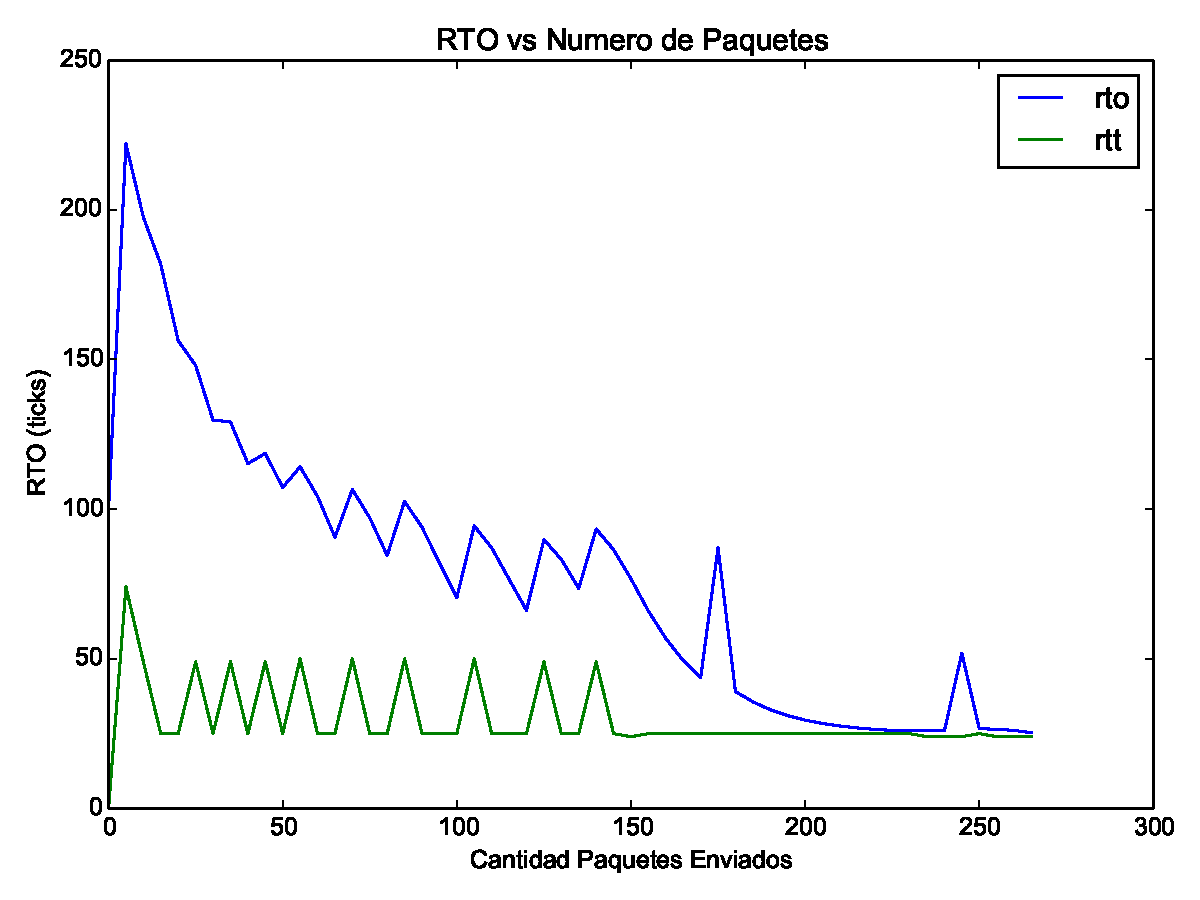
\includegraphics[width=0.32\textwidth]{imagenes/rtt_vs_n_2_4.pdf}
		    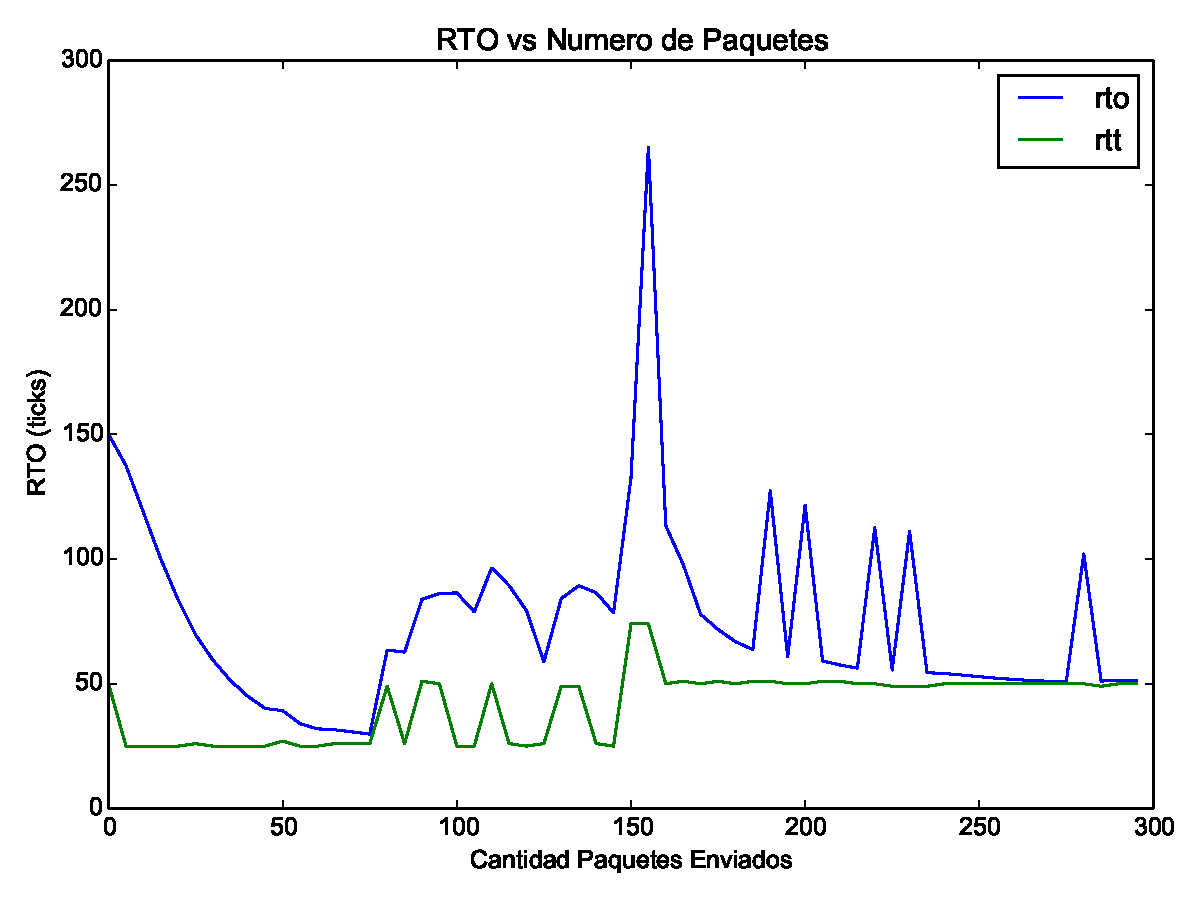
\includegraphics[width=0.32\textwidth]{imagenes/congestion_50_2_4.pdf}
		    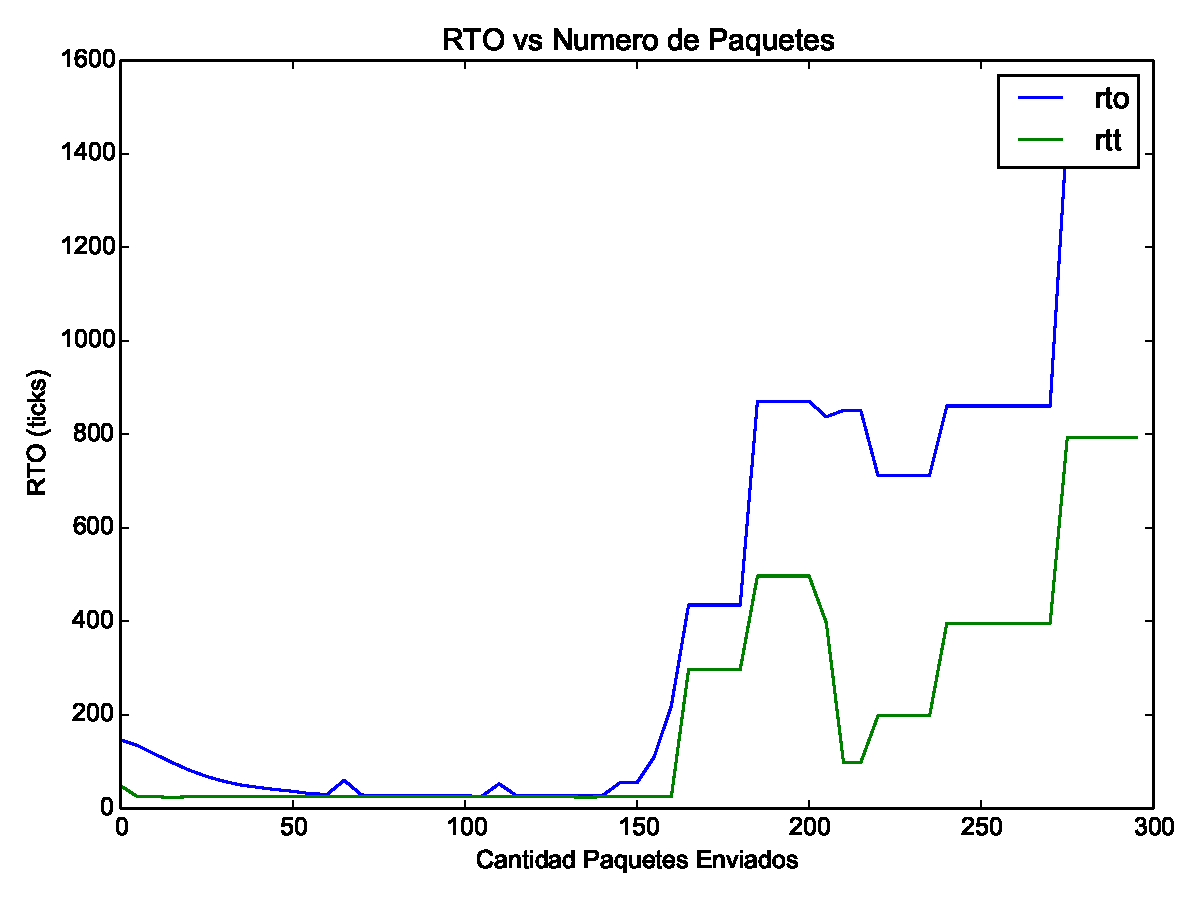
\includegraphics[width=0.32\textwidth]{imagenes/congestion_100_2_4.pdf}

            \caption{Escenario 1}
	
        \end{figure}          
  
        El \emph{Escenario 2} muestra el resultado en una red con
        par\'aemtros: $\alpha={{1}\over{8}}$, $\beta={{1}\over{2}}$ 
        cuando no se congestiona, cuando la congesti\'on causa el doble de
        delay, y cuando causa el cuadruple.

        \begin{figure}[H]
            \center
	        
		    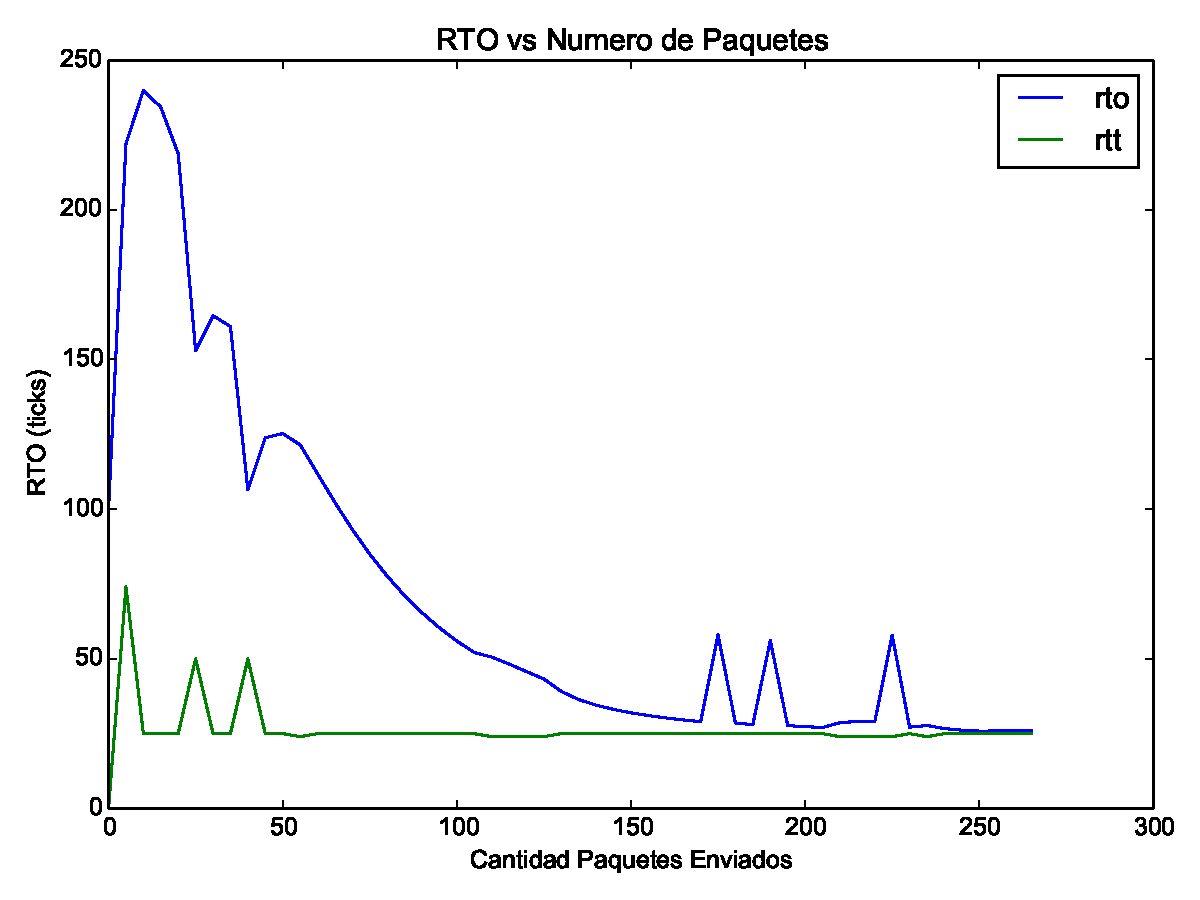
\includegraphics[width=0.32\textwidth]{imagenes/rtt_vs_n_8_2.pdf}
		    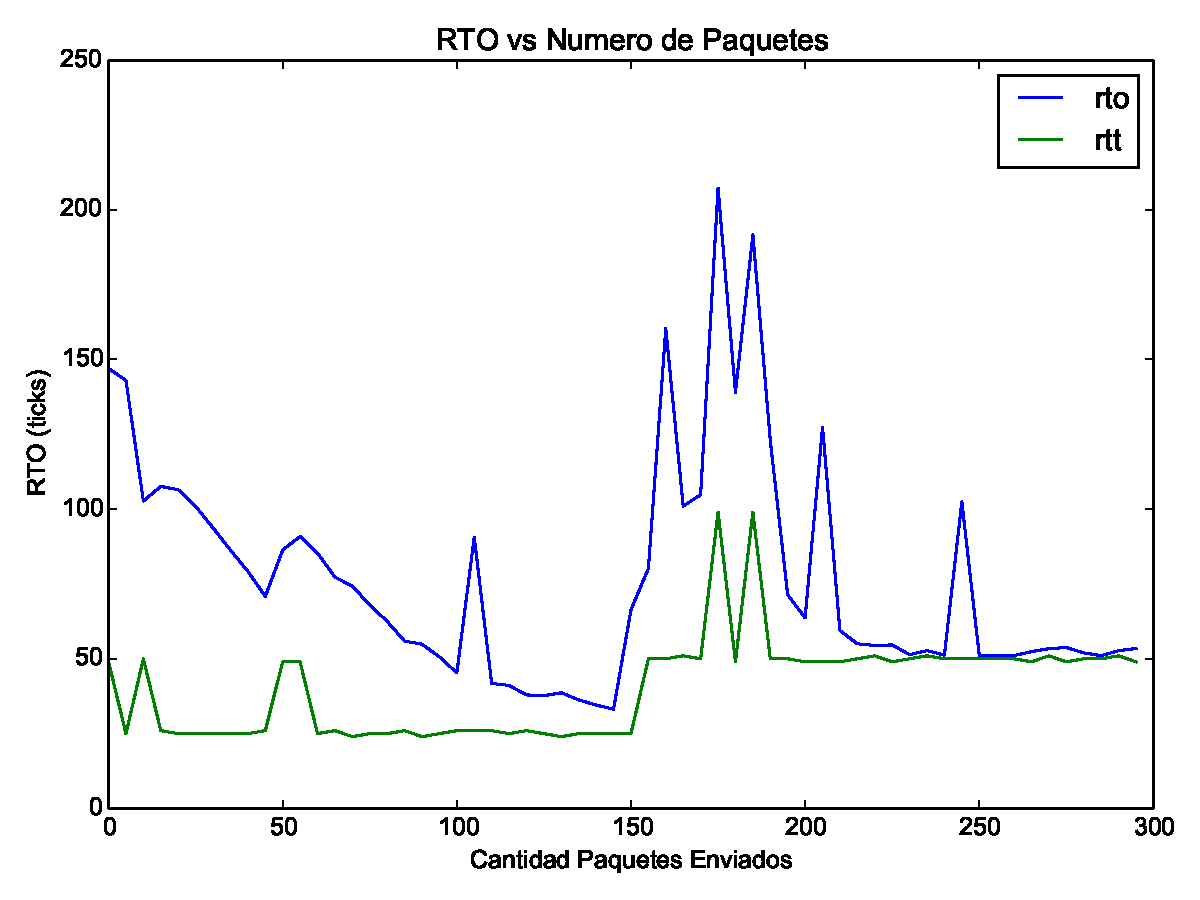
\includegraphics[width=0.32\textwidth]{imagenes/congestion_50_8_2.pdf}
		    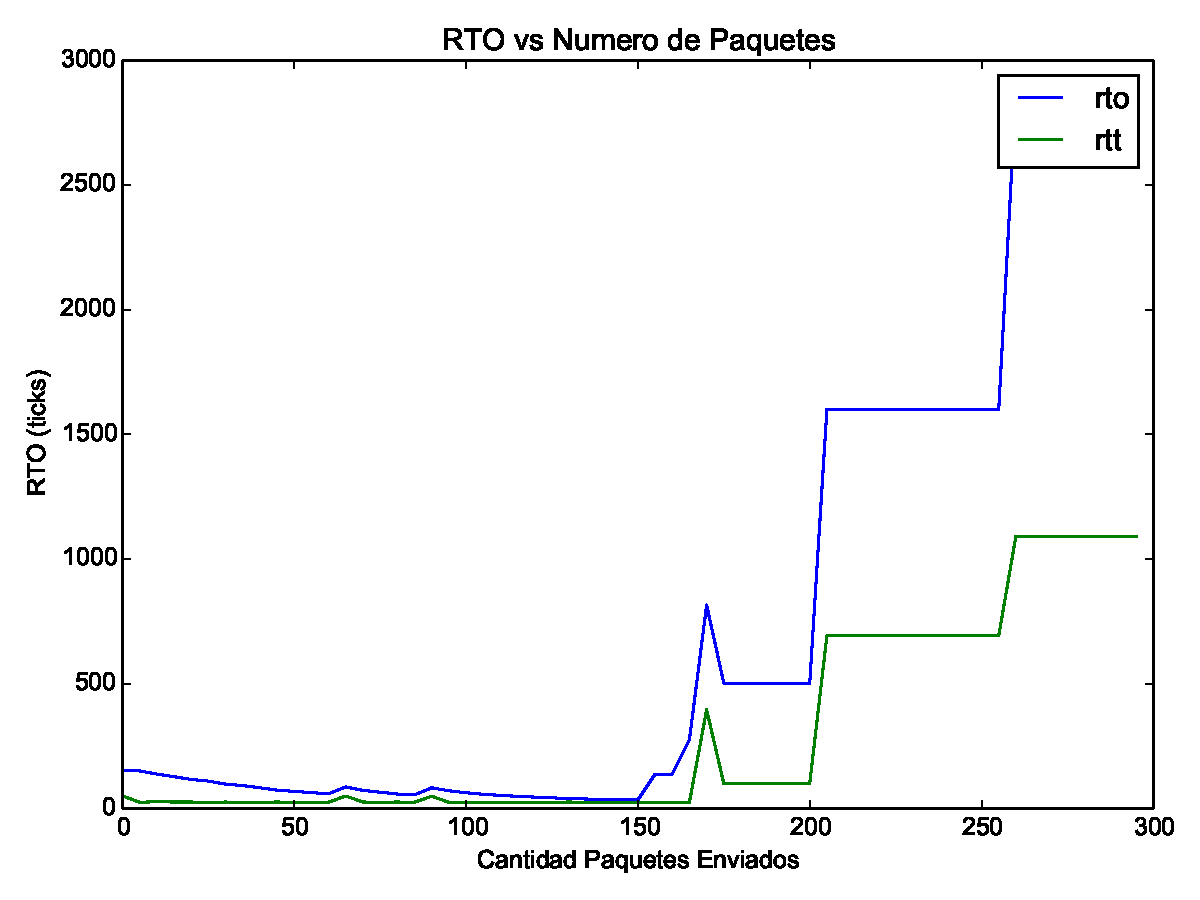
\includegraphics[width=0.32\textwidth]{imagenes/congestion_100_8_2.pdf}

            \caption{Escenario 1}
	
        \end{figure}          

        En ambos casos sucedi\'o que al duplicar el valor del delay el 
        mensaje n\'umero 101 debi\'o ser retransmitido. A su vez, cuando 
        se cuadruplic\'o el valor de la red, el mensaje n\'umero 101 debi\'o
        ser retransmitido dos veces. 
        Tambi\'en se puede notar que en ambos casos luego de cuadruplicarse
        el delay no se logr\'o volver a un \rto{} cercano a el \rtt{} real.


    \subsection{Tiempo total de transmisi\'on en entorno con p\'erdidas}
        
        Para este experimento se configur\'o un escenario en el cual el 
        cliente env\'ia 300 mensajes al servidor, pasados los 150 el delay
        se incrementa de \textit{25 ticks} a \textit{50 ticks}. A su vez,
        la probabilidad de perder un paquete es de 0.1.
        Luego, utilizando wireshark, se calcul\'o el tiempo que dur\'o la
        conexi\'on en base a los paquetes capturados y su timestamp.
        
        Para los valores de $\alpha=0$ y $\beta=0$ el tiempo fue 42,19 seg,
        para los valores propuestos por el RFC el tiempo promedio fue
        41,67 seg, para $\alpha=0.15$ y $\beta=0.2$ 42,39 seg, finalmente  
        para $\alpha=1$ y $\beta=1$ el tiempo fue 44,34 seg.
        



\section{Conclusiones}

Todos los experimentos demostraron lo susceptible que es la medici\'on de
RTO a los par\'ametros de la red, as\'i como tambi\'en a los par\'ametros
utilizados para estimarlo. 

Primero vimos que cambiar los valores de $\alpha$ y $\beta$ modifican
significativamente el valor estimado de \rto{}, al experimentar con valores
muy peque\~nos, los cálculos no se adaptan de forma realista a las
variaciones en los valores de RTT reales. Por el contrario, al tomar
valores muy altos los mismos se ven demasiado influenciados por
fluctuaciones temporales, dando como resultado valores demasiado altos o
demasiado peque\~nos en comparación con el RTT real. 

Luego vimos como los valores de $\alpha$ y $\beta$ modifican la cantidad
de retransmisiones, cabe destacar que las \textit{Figuras 5 y 6} son parte
de un experimento en el cual no se simul\'o perdida de paquetes, sin embargo
, hubo retransmisiones. Esto se debe a que cuando el \rto{} se acerca al 
\rtt{} estimado es muy sensible a cambios internos de la pc, recordemos que
los procesos de cliente y servidor est\'an funcionando dentro de un sistema
operativo hogareño. 

Por \'ultimo, vimos como el c\'alculo del \rto{} afecta a la transmisi\'on
total de una conexi\'on. Podemos ver que entre el primer resultado hay casi
dos segundos de diferencia, teniendo en cuenta que el tiempo para enviar un 
mensaje entre ambos nodos es menor a 0.1 seg, podemos ver que la diferencia
de performance es notable.

Para concluir queremos agregar que el valor que mejor funcion\'o en los 
experimentos fue el propuesto por el RFC, consiguiendo aproximarnos con $\alpha=0.15$ y $\beta=0.2$. 


%\section{Referencias}
%\begin{itemize}
%	\item \textbf{Computer Networks: A Systems Approach}, \textit{Larry L. Peterson and Bruce S. Davie.}
%	\item \textbf{Computer Networks}, \textit{Andrew S. Tanenbaum}
%%	\item \textbf{http://submarinecablemap.com/}
%%	\item \textbf{Special-Purpose IP Address Registries} (RFC 6890), \textit{Internet Engineering Task Force (IETF)}
%%	\item \textbf{An Ethernet Address Resolution Protocol or Converting Network Protocol Addresses to 48.bit Ethernet Address for Transmission on Ethernet Hardware} (RFC 826), \textit{David C. Plummer}
%\end{itemize}

\end{document}
